\section{Cameras}\label{chap:cameras}

Cameras are the sensors that capture the richest information about the scene, but they only give us a 2D image of a 3D world.
In this chapter we see how a camera forms an image, how to describe it mathematically (intrinsics and extrinsics), how to correct the lens distortion with the calibration, and how to extract and track interesting points across frames.

\subsection{The pinhole camera model}
\noindent\begin{minipage}[c]{0.6\textwidth}
The \textbf{pinhole camera} model describes the relationship between the coordinates of a point in 3D space and its projection onto the \textbf{image plane}.
The camera aperture is modelled as a single point (the \textbf{pinhole}, or optical centre): every ray of light coming from the scene passes through it and hits the image plane, producing an inverted image.
The distance between the aperture and the image plane is the \textbf{focal length} $f$.
\end{minipage}\hfill
\begin{minipage}[c]{0.36\textwidth}
    \centering
    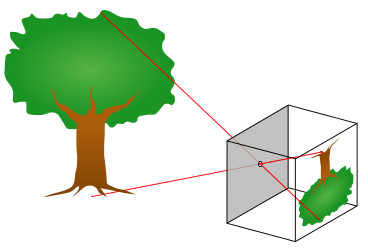
\includegraphics[width=\linewidth]{images/C8_1.png}
    \captionof{figure}{Pinhole camera}
\end{minipage}

\vspace{6pt}A camera captures a 3D scene and projects it onto a 2D image. With the pinhole model, a 3D point $(X, Y, Z)$ in world coordinates is projected to the pixel $(u, v)$ as:
\[
s \begin{bmatrix} u \\ v \\ 1 \end{bmatrix} = K\,[R \mid t] \begin{bmatrix} X \\ Y \\ Z \\ 1 \end{bmatrix} = P \begin{bmatrix} X \\ Y \\ Z \\ 1 \end{bmatrix}
\]
where $[R \mid t]$ is the \textbf{extrinsic matrix} (the camera pose), $K$ is the \textbf{intrinsic matrix} (focal length and principal point), $P = K[R \mid t]$ is the \textbf{projection matrix}, which combines both, and $s$ is a scale factor equal to the depth of the point.
The projection is done in two steps: first the point is moved from the world frame to the camera frame (extrinsics), then it is projected onto the image (intrinsics).

\subsubsection{Camera extrinsics}
The \textbf{extrinsics} describe the \textbf{position and orientation} of the camera in the world frame.
They are a rigid body transformation $[R \mid t] \in SE(3)$, where $R \in SO(3)$ is the rotation from the world frame to the camera frame and $t \in \mathbb{R}^3$ is the translation from the world origin to the camera origin.
A point is transformed from world to camera coordinates as:
\[
P_c = R\,P_w + t
\]

\subsubsection{Camera intrinsics}
The \textbf{intrinsics} define the mapping from the camera coordinates $(X_c, Y_c, Z_c)$ to the image pixels $(u, v)$, and they are collected in the \textbf{intrinsic matrix}:
\[
K = \begin{bmatrix} f_x & 0 & c_x \\ 0 & f_y & c_y \\ 0 & 0 & 1 \end{bmatrix}
\qquad\qquad
\begin{bmatrix} u \\ v \\ 1 \end{bmatrix} = K \begin{bmatrix} X_c / Z_c \\ Y_c / Z_c \\ 1 \end{bmatrix}
\]
where $f_x$, $f_y$ are the \textbf{focal lengths in pixels} (they may differ if the pixels are not square) and $c_x$, $c_y$ are the coordinates of the \textbf{principal point}, i.e.\ where the optical axis hits the image (roughly the image centre).
Dividing by $Z_c$ is what makes the projection a \textbf{perspective} projection: the further an object is, the smaller it appears. It is also why a single camera loses the depth: all the points along the same ray are projected to the same pixel.

\begin{figure}[H]
    \centering
    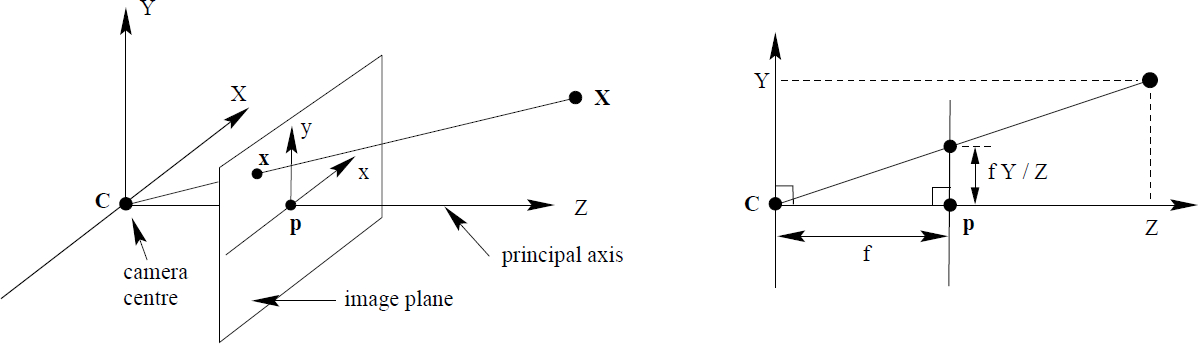
\includegraphics[width=0.7\textwidth]{images/C8_2.png}
    \caption{Projection of a point $X$ onto the image plane: by similar triangles, $y = fY/Z$}
\end{figure}

\begin{examplebox}[Projecting a 3D point]
Consider a camera with
\[
K = \begin{bmatrix} 800 & 0 & 320 \\ 0 & 800 & 240 \\ 0 & 0 & 1 \end{bmatrix}, \qquad R = I, \qquad t = \begin{bmatrix} 0 \\ 0 \\ -5 \end{bmatrix}
\]
and the 3D point $P_w = [1, 2, 10]^T$. First we move it to the camera frame:
\[
P_c = R\,P_w + t = [1, 2, 5]^T
\]
Then we project it to pixels:
\[
u = f_x \frac{X_c}{Z_c} + c_x = 800 \cdot \tfrac{1}{5} + 320 = 480 \qquad\quad
v = f_y \frac{Y_c}{Z_c} + c_y = 800 \cdot \tfrac{2}{5} + 240 = 560
\]
\end{examplebox}

\subsection{Lens distortion}
Real cameras use \textbf{lenses} to focus more light and obtain better images, but lenses are not perfect and introduce \textbf{distortion}. There are two main types.

\textbf{Radial distortion} bends straight lines, and it is common in wide-angle lenses. It depends on the distance $r$ from the image centre, with $r^2 = x^2 + y^2$:
\[
x_{dist} = x\,(1 + k_1 r^2 + k_2 r^4 + k_3 r^6) \qquad\quad
y_{dist} = y\,(1 + k_1 r^2 + k_2 r^4 + k_3 r^6)
\]
\textbf{Tangential distortion} is caused by the lens not being perfectly aligned with the sensor:
\[
x_{dist} = x + \left[2p_1 xy + p_2(r^2 + 2x^2)\right] \qquad\quad
y_{dist} = y + \left[p_1(r^2 + 2y^2) + 2p_2 xy\right]
\]

\begin{figure}[H]
    \centering
    \begin{subfigure}{0.45\textwidth}
        \centering
        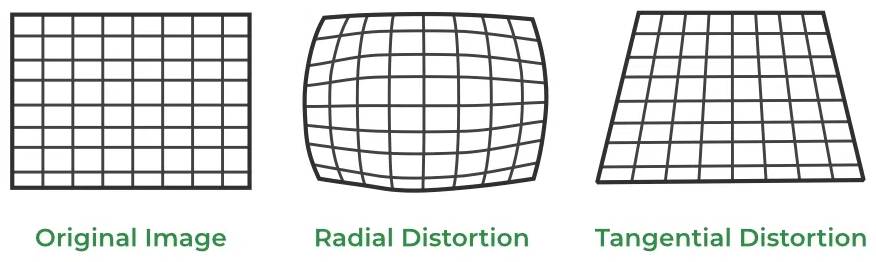
\includegraphics[width=\linewidth]{images/C8_3.png}
        \caption{Radial and tangential distortion}
    \end{subfigure}\hfill
    \begin{subfigure}{0.5\textwidth}
        \centering
        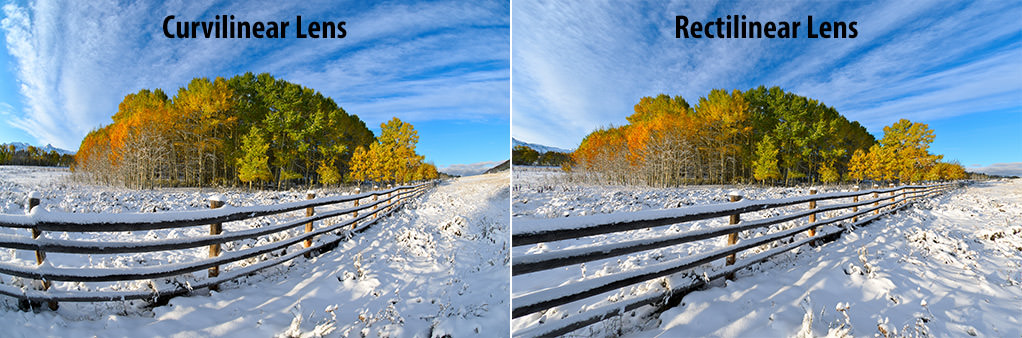
\includegraphics[width=\linewidth]{images/C8_4.png}
        \caption{The same scene with a distorted and a corrected lens}
    \end{subfigure}
    \caption{Lens distortion}
\end{figure}

The \textbf{camera calibration} estimates the coefficients $k_i$ and $p_i$, and for accurate 3D reconstruction and measurements the distortion must always be compensated.

\subsubsection{Other camera models}
Besides the pinhole model, other camera models exist:
\begin{compactitemize}
    \item \textbf{Fisheye camera}: ultra-wide-angle lens with a strong radial distortion, which projects a whole hemisphere onto the image plane;
    \item \textbf{Omnidirectional camera}: 360° field of view, often obtained with mirrors (catadioptric systems); useful in robotics and surveillance;
    \item \textbf{Telecentric camera}: the rays are parallel to the optical axis, so there is no perspective distortion; used in industrial measurements.
\end{compactitemize}

\subsection{Camera intrinsic calibration}
The purpose of the \textbf{intrinsic calibration} is to determine the intrinsic parameters of a camera, to obtain an accurate 3D-to-2D projection.
The parameters to estimate are the focal lengths $f_x$, $f_y$, the principal point $c_x$, $c_y$, the skew $s$ (usually zero) and the distortion coefficients $k_1, k_2, k_3, p_1, p_2$.
They are needed to correct the lens distortion, to obtain accurate 3D reconstructions and for sensor fusion.

\noindent\begin{minipage}[c]{0.62\textwidth}
The common procedure is:
\begin{enumerate}
    \item capture multiple images of a \textbf{calibration pattern} (e.g.\ a checkerboard) at different orientations;
    \item detect the feature points (corners or tags) in each image;
    \item since the 3D geometry of the pattern is known, solve for the intrinsic parameters using the camera model $s[u, v, 1]^T = K[R \mid t][X_w, Y_w, Z_w, 1]^T$;
    \item optionally, estimate the lens distortion coefficients.
\end{enumerate}
Common tools are OpenCV (\texttt{cv::calibrateCamera()}), the MATLAB Camera Calibration Toolbox and the ROS calibration packages (e.g.\ Kalibr).
\end{minipage}\hfill
\begin{minipage}[c]{0.34\textwidth}
    \centering
    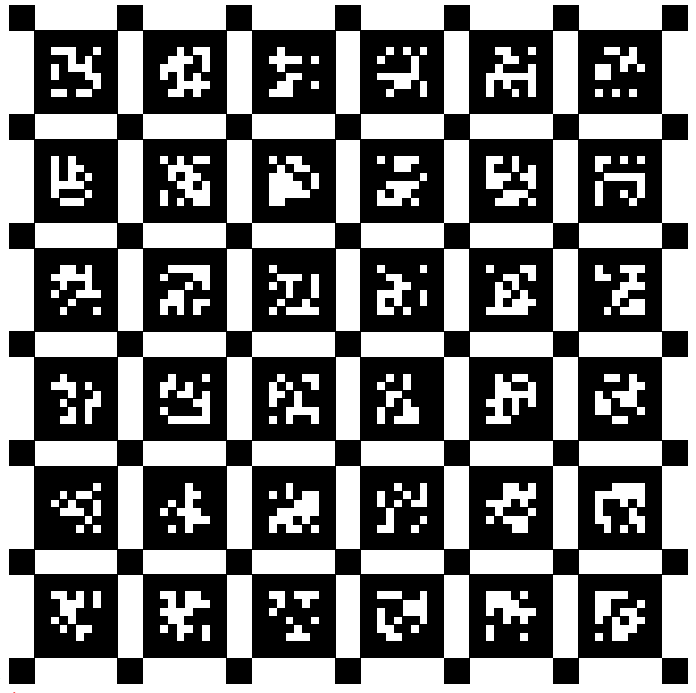
\includegraphics[width=0.48\linewidth]{images/C8_5.png}\hfill
    
\includegraphics[width=0.48\linewidth]{images/C8_6.png}
    \captionof{figure}{Calibration targets: AprilGrid and checkerboard}
\end{minipage}

\subsubsection{Point undistortion}
Because of the lens distortion, the measured pixel coordinates $(u_d, v_d)$ are distorted. The goal of the \textbf{undistortion} is to compute the coordinates $(u, v)$ that correspond to the ideal pinhole projection:
\begin{enumerate}
    \item convert the distorted pixels to \textbf{normalized image coordinates}: $x_d = \frac{u_d - c_x}{f_x}$, $y_d = \frac{v_d - c_y}{f_y}$;
    \item apply the \textbf{inverse distortion model} to correct the radial and tangential distortion, obtaining $(x, y)$;
    \item convert back to pixel coordinates with the intrinsics: $u = f_x x + c_x$, $v = f_y y + c_y$.
\end{enumerate}
The result are undistorted pixel coordinates, suitable for accurate 3D reconstruction.

\subsection{Keypoints extraction}
\textbf{Keypoints} are distinct and repeatable points of an image, which can be identified again and are robust to changes in scale, rotation, illumination and viewpoint.
They can be \textbf{corners} (points with a large intensity change in two directions), \textbf{blobs} (regions with locally uniform intensity) or \textbf{edges} (points along the image gradients).

Common detection algorithms are Shi-Tomasi, the Harris corner detector, FAST, SIFT (Scale-Invariant Feature Transform), SURF (Speeded Up Robust Features), ORB (Oriented FAST and Rotated BRIEF) and deep learning methods such as SuperPoint.

\subsubsection{FAST}
\noindent\begin{minipage}[c]{0.55\textwidth}
\textbf{FAST} (Features from Accelerated Segment Test) works as follows:
\begin{enumerate}
    \item consider a candidate pixel $p$ and a circle of 16 pixels around it;
    \item $p$ is a corner if at least $N$ \textbf{contiguous} pixels of the circle are all brighter, or all darker, than $p$ by a threshold $t$;
    \item typically $N = 12$, while $t$ is chosen based on the image contrast;
    \item finally, non-maximum suppression keeps only the strongest corners.
\end{enumerate}
\end{minipage}\hfill
\begin{minipage}[c]{0.41\textwidth}
    \centering
    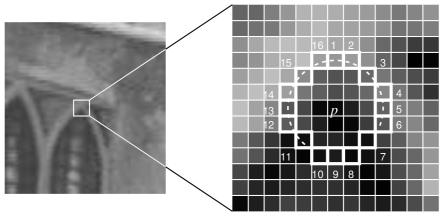
\includegraphics[width=\linewidth]{images/C8_7.png}
    \captionof{figure}{The 16-pixel circle of FAST}
\end{minipage}

\vspace{6pt}FAST is \textbf{very fast}, suitable for real-time applications, and simple to implement. However, it is not scale-invariant, it is sensitive to noise and its threshold must be tuned.

\subsection{Optical flow}
\textbf{Optical flow} is the apparent motion of the brightness patterns in an image sequence: it represents how the pixels move from one frame to the next,
\[
I(x, y, t) = I(x + u, y + v, t + 1)
\]
where $(u, v)$ is the displacement of the pixel at $(x, y)$.
Common algorithms are Lucas-Kanade and deep learning methods (SuperGlue, FlowNet, RAFT).

\begin{figure}[H]
    \centering
    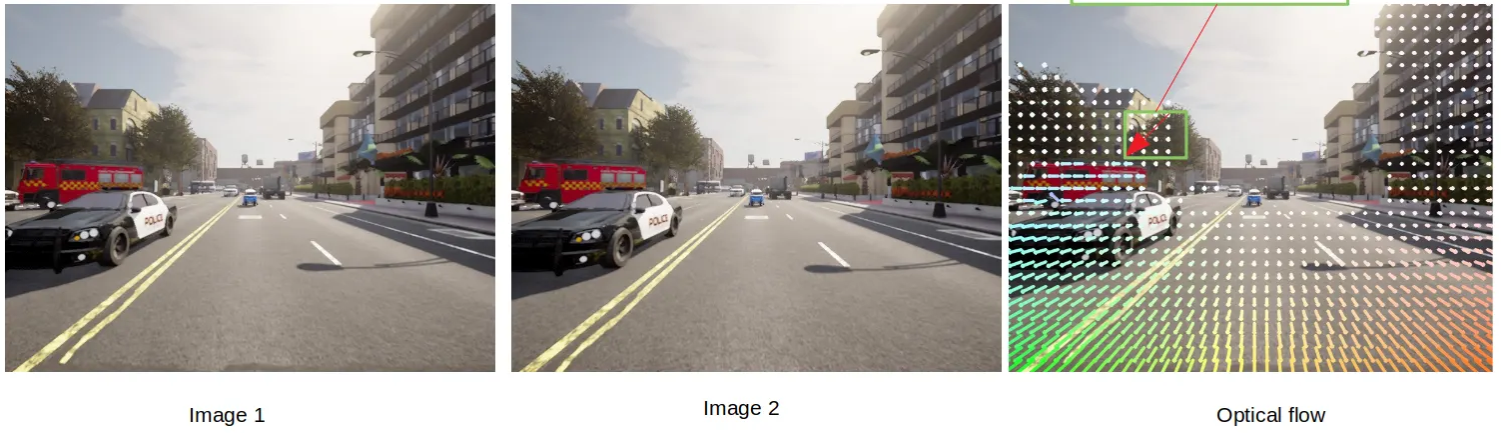
\includegraphics[width=0.8\textwidth]{images/C8_8.png}
    \caption{Two consecutive frames and the resulting optical flow}
\end{figure}

\subsubsection{Lucas-Kanade}
The \textbf{Lucas-Kanade} method is based on three assumptions:
\begin{compactitemize}
    \item \textbf{brightness constancy}: the intensity of a pixel does not change while it moves, $I(x, y, t) = I(x + u, y + v, t + 1)$;
    \item \textbf{small motion}: the displacement is small, so the equation can be linearized with a Taylor expansion, obtaining $I_x u + I_y v + I_t = 0$;
    \item \textbf{local motion consistency}: neighbouring pixels have a similar flow.
\end{compactitemize}
A single pixel gives one equation in two unknowns, which is not enough. Thanks to the third assumption, we use all the $n$ pixels $p_i$ of a small window around the point, obtaining an over-determined system solved with least squares:
\[
\begin{bmatrix} I_x(p_1) & I_y(p_1) \\ \vdots & \vdots \\ I_x(p_n) & I_y(p_n) \end{bmatrix}
\begin{bmatrix} u \\ v \end{bmatrix}
= - \begin{bmatrix} I_t(p_1) \\ \vdots \\ I_t(p_n) \end{bmatrix}
\]
where $I_x$, $I_y$, $I_t$ are the derivatives of the image in space and time.
The method is simple and fast and works well for sparse features, but it assumes small motion and it is sensitive to noise and illumination changes.

\subsection{Tracking points with keypoints and optical flow}
Combining the two techniques we can \textbf{track} salient points across the frames of a video:
\begin{enumerate}
    \item \textbf{Keypoint detection}: identify distinctive points in the first frame with a detector like FAST, ORB or Shi-Tomasi;
    \item \textbf{Optical flow estimation}: compute the motion vectors of the keypoints between consecutive frames, e.g.\ with Lucas-Kanade;
    \item \textbf{Update positions}: use the flow vectors to update the keypoint positions in the next frame;
    \item \textbf{Iterate} over the whole sequence.
\end{enumerate}
Applications are visual odometry, SLAM and object tracking.


The next question is: how can we use this 2D information to \textbf{recover the 3D structure} of the scene and the motion of the camera?

\subsection{Camera motion reconstruction}
Given two images of the same world, taken by two different cameras (or by the same camera in two different positions), we want to recover \textbf{where the second camera is with respect to the first one}.

\subsubsection{What can be recovered from an image pair}
\noindent\begin{minipage}[c]{0.55\textwidth}
From two images we can recover:
\begin{compactitemize}
    \item the \textbf{rotation} of the second camera with respect to the first one (3 parameters);
    \item the \textbf{direction} of the line connecting the two centres of projection (2 parameters).
\end{compactitemize}
That is 5 parameters, and not 6: given two images, the scene can be reconstructed only up to a \textbf{similarity transform}, so it is not possible to recover the \textbf{scale} of the world.
A small object close to the cameras and a big object far away, with the cameras proportionally further apart, produce exactly the same images.
\end{minipage}\hfill
\begin{minipage}[c]{0.41\textwidth}
    \centering
    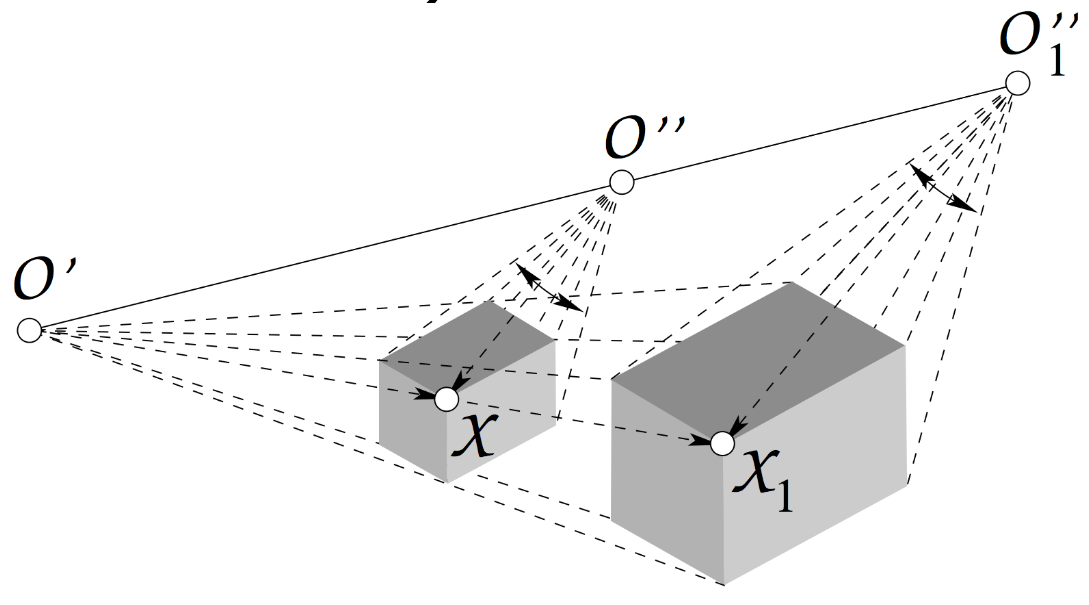
\includegraphics[width=\linewidth]{images/C8_9.png}
    \captionof{figure}{Scale ambiguity: $X$ seen from $O', O''$ and $X_1$ seen from $O', O''_1$ give the same images}
\end{minipage}

\subsubsection{Epipolar geometry}
\textbf{Epipolar geometry} describes the geometric relationship between two cameras observing the same 3D scene.
A point $P$ is seen in the two images as $p$ and $p'$, and the camera centres $O_1$, $O_2$, the point $P$ and its two projections all lie on the same plane, the \textbf{epipolar plane}.

The key concepts are:
\begin{compactitemize}
    \item \textbf{epipoles} $e$, $e'$: the intersections of the line connecting the two camera centres (the \textbf{baseline}) with the image planes;
    \item \textbf{epipolar lines}: the lines in each image on which the projection of a 3D point must lie. Given $p$ in the first image, its correspondence $p'$ must lie on the epipolar line through $e'$, so the search for correspondences becomes 1D.
\end{compactitemize}

\begin{figure}[H]
    \centering
    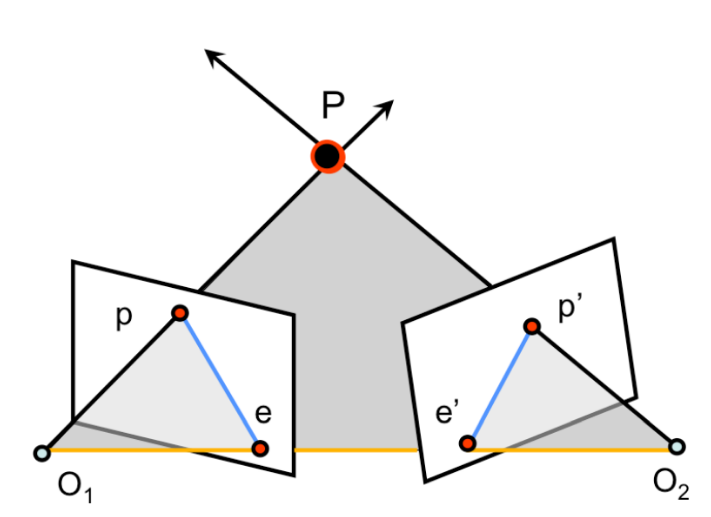
\includegraphics[width=0.3\textwidth]{images/C8_10.png}
    \caption{Epipolar geometry}
\end{figure}

Let's write this constraint mathematically. The normalized directions of the vectors $O_1P$ and $O_2P$, expressed in the world frame, are
\[
{}^n p = R_{W\leftarrow1}\,K_1^{-1}\,p \qquad\qquad {}^n p' = R_{W\leftarrow2}\,K_2^{-1}\,p'
\]
and the \textbf{baseline} vector is $b = t_2 - t_1$.
These three vectors are \textbf{coplanar}, so their triple product is zero:
\[
{}^n p \cdot (b \times {}^n p') = 0
\quad\Rightarrow\quad {}^n p^T\,[b]_\times\,{}^n p' = 0
\quad\Rightarrow\quad (R_{W\leftarrow1}K_1^{-1}p)^T\,[b]_\times\,R_{W\leftarrow2}K_2^{-1}p' = 0
\]
\[
p^T \underbrace{K_1^{-T}\,R_{1\leftarrow W}\,[b]_\times\,R_{W\leftarrow2}\,K_2^{-1}}_{F}\,p' = 0
\quad\Rightarrow\quad p^T F\,p' = 0
\]
where we used $R_{W\leftarrow1}^T = R_{1\leftarrow W}$ and the cross product written with the skew-symmetric matrix $[b]_\times$ seen in the previous chapter.

\subsubsection{Fundamental and essential matrix}
The matrix
\[
F = K_1^{-T}\,R_{1\leftarrow W}\,[b]_\times\,R_{W\leftarrow2}\,K_2^{-1}
\]
is called \textbf{fundamental matrix}, and it expresses the coplanarity constraint between two corresponding points: $p^T F p' = 0$.
It contains all the available information about the relative orientation of two images taken by \textbf{uncalibrated} cameras.

If the cameras are \textbf{calibrated}, $K_1$ and $K_2$ are known, and we can work directly with the normalized coordinates ${}^k p = K_1^{-1}p$ and ${}^k p' = K_2^{-1}p'$.
The constraint becomes ${}^k p^T E\,{}^k p' = 0$, where
\[
E = R_{1\leftarrow W}\,[b]_\times\,R_{W\leftarrow2}
\]
is the \textbf{essential matrix}.
If we take the first camera as the global reference frame ($R_{1\leftarrow W} = I$, $t_{1\leftarrow W} = 0$), the essential matrix becomes
\[
E = [t_{1\leftarrow2}]_\times\,R_{1\leftarrow2}
\]
which contains exactly the \textbf{relative motion} between the two cameras.

\begin{infobox}[F vs E]
The fundamental matrix works directly on pixels and does not need the calibration; the essential matrix works on normalized coordinates and needs $K$, but it contains directly the relative rotation and translation. The two are related by $F = K_1^{-T}\,E\,K_2^{-1}$. In an AD system the cameras are calibrated, so we use $E$.
\end{infobox}

\paragraph{Computation: the 8-point algorithm}
Given a set of corresponding 2D points $\{(x'_i, x''_i)\}$ in the two images, the fundamental (or essential) matrix can be computed with the \textbf{8-point algorithm}.
Each correspondence gives one coplanarity equation $x_i'^T F x''_i = 0$, which is linear in the 9 entries of $F$.
Stacking 8 of them (the matrix is defined up to a scale, so 8 unknowns are left) we obtain a linear system:
\[
\begin{bmatrix} (x''_0 \otimes x'_0)^T \\ \vdots \\ (x''_7 \otimes x'_7)^T \end{bmatrix}
\begin{bmatrix} F_{11} & F_{12} & \cdots & F_{33} \end{bmatrix}^T = 0
\]
More complex algorithms need fewer points (the 7-point and the 5-point algorithms).

\paragraph{Robust computation with RANSAC}
Real correspondences are noisy and contain wrong matches (outliers), so \textbf{RANSAC} is used to compute $F$ or $E$ robustly:
\begin{enumerate}
    \item detect and match feature points between the two images;
    \item randomly select the minimum set of 8 correspondences;
    \item compute a candidate $F$ with the 8-point algorithm;
    \item evaluate the error of all the correspondences, and classify as \textbf{inliers} those with an error below $\epsilon$;
    \item repeat for many iterations, keeping the $F$ with the largest consensus set;
    \item recompute $F$ using all the inliers (least squares refinement).
\end{enumerate}

\paragraph{Ill-posed cases}
The computation becomes \textbf{ill-posed} when all the detected points lie on a \textbf{plane}, or when there is \textbf{no translation} between the two cameras (pure rotation: the baseline is zero, so there is no epipolar plane).

\subsubsection{Relative pose recovery}
Given the essential matrix $E$, we can \textbf{decompose} it to recover the relative motion between the two cameras.
Since the scale cannot be recovered, the translation is only a \textbf{direction} ($\|t_{1\leftarrow2}\| = 1$).
The decomposition has \textbf{4 admissible solutions}, but only in one of them the reconstructed points are \textbf{in front of both cameras}.

\begin{figure}[H]
    \centering
    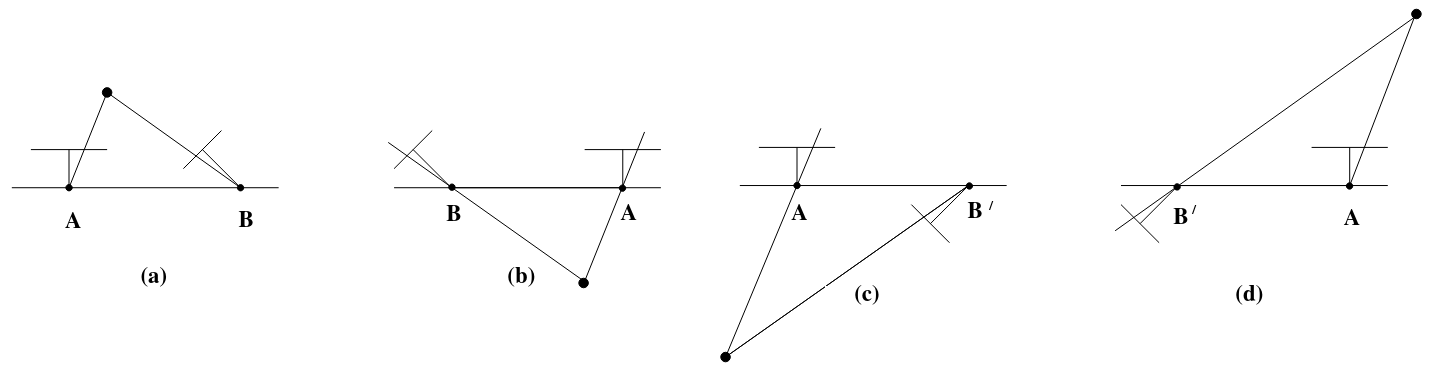
\includegraphics[width=0.7\textwidth]{images/C8_11.png}
    \caption{The four possible decompositions of $E$: only in (a) the point is in front of both cameras}
\end{figure}

\paragraph{Linear triangulation}
To check which solution is correct we need the 3D points, which we obtain by \textbf{triangulation}.
In each image we have a measurement, $x = PX$ and $x' = P'X$, where $P$, $P'$ are the projection matrices.
Since $x$ and $PX$ are parallel, their cross product is zero, $x \times (PX) = 0$, which gives (with $P_i^T$ the rows of $P$):
\[
\begin{cases}
x\,(P_3^T X) - (P_1^T X) = 0 \\
y\,(P_3^T X) - (P_2^T X) = 0 \\
x\,(P_2^T X) - y\,(P_1^T X) = 0
\end{cases}
\]
The third equation is a linear combination of the first two, so we use only the first two for each image, obtaining the system
\[
A X = 0 \quad\rightarrow\quad
\begin{bmatrix} x P_3^T - P_1^T \\ y P_3^T - P_2^T \\ x' P_3'^T - P_1'^T \\ y' P_3'^T - P_2'^T \end{bmatrix}
\begin{bmatrix} X \\ Y \\ Z \\ W \end{bmatrix} = 0
\]
which is solved for the homogeneous 3D point (e.g.\ with SVD).

\paragraph{Cheirality check}
A triangulated point is valid only if it is \textbf{in front of both cameras}, i.e.\ its $Z$ coordinate is positive in both camera frames.
So we decompose $E$, triangulate the points with each of the 4 solutions, and keep the one for which most of the triangulated points are in front of both cameras.

\subsubsection{Recap: motion from an image pair}
Given two images, the relative motion is obtained as follows:
\begin{enumerate}
    \item compute salient \textbf{keypoints} in the first image (e.g.\ FAST);
    \item \textbf{match} them in the second image with optical flow (e.g.\ Lucas-Kanade);
    \item remove the \textbf{distortion} of the points;
    \item compute the \textbf{essential matrix} $E$ with RANSAC and remove the outliers;
    \item \textbf{decompose} $E$ to obtain the possible motions;
    \item \textbf{triangulate} the inliers;
    \item perform the \textbf{cheirality check} on the triangulated points to select the correct relative motion.
\end{enumerate}

\subsubsection{Perspective-n-Point (PnP)}
Once we have some 3D points, we can localize a new camera directly, without the essential matrix.
The goal of \textbf{Perspective-n-Point} (PnP) is to estimate the \textbf{pose} of the camera (rotation $R$ and translation $t$) given a set of $n$ known 3D points $P_i$ in world coordinates and their corresponding 2D projections $p_i$ in the image.
The minimum requirement is 3 points (P3P), but usually $n \gg 3$ for robustness.
Unlike the essential matrix, PnP uses known 3D points, so the recovered translation keeps the \textbf{scale} of those points.

\begin{figure}[H]
    \centering
    \begin{subfigure}{0.42\textwidth}
        \centering
        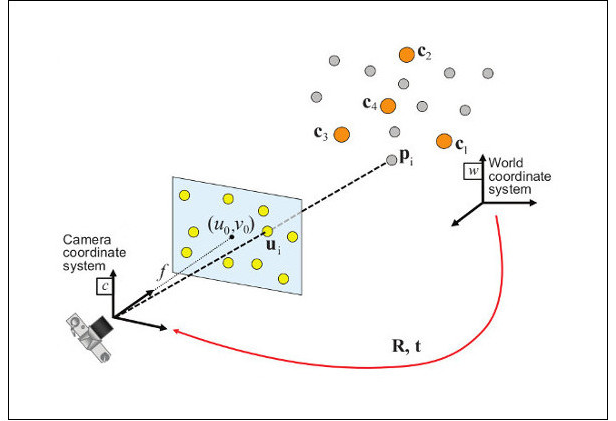
\includegraphics[width=\linewidth]{images/C8_12a.png}
    \end{subfigure}
    \hspace{1cm}
    \begin{subfigure}{0.42\textwidth}
        \centering
        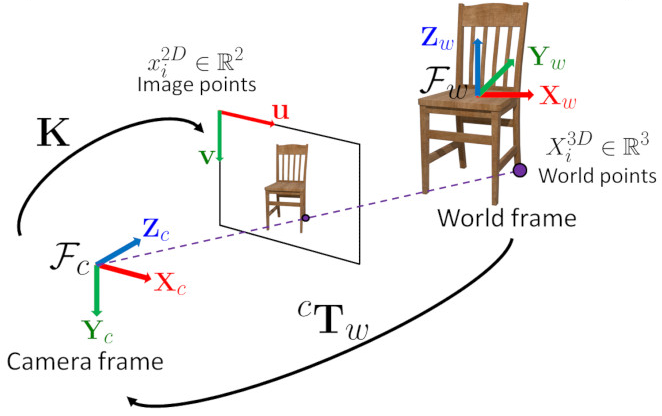
\includegraphics[width=\linewidth]{images/C8_12b.png}
    \end{subfigure}
    \caption{PnP: from 3D world points and their 2D projections to the camera pose}
\end{figure}

\subsubsection{Recap: motion from three images}
With three images, we first apply the previous procedure to the first two, and then:
\begin{enumerate}
    \setcounter{enumi}{7}
    \item \textbf{match} the keypoints of the second image into the third one with optical flow;
    \item use \textbf{PnP} with the 3D points triangulated from the first two images and their undistorted 2D correspondences in the third image, to compute the position and orientation of the third camera.
\end{enumerate}
In this way all the three poses share the same (unknown) scale, fixed by the first pair.
The natural next question is: how can we scale this approach to \textbf{more than 3 images}?
